\subsection{Caratheodory Measurability and Lebesgue Measure}
\begin{definition} \label{def:outer-measure-and-rudin-measurable-sets} \hlt{Outer Measure and $\mu$-Measurable Sets}\\
Let $\mu$ be additive, regular, nonnegative, and finite on $\mathcal{E}$.\\
For $E\subseteq\R^p$, define $\mu^\ast(E)\defeq\inf\sum\limits_{n=1}^{\infty}\mu(A_n)$, where infimum is over open elementary covers $E\subseteq\bigcup\limits_{n=1}^{\infty}A_n$.\\
For $A,B\subseteq\R^p$, set $A\triangle B\defeq(A\setminus B)\cup(B\setminus A)$ and $d_\mu(A,B)\defeq\mu^\ast(A\triangle B)$.\\
A set is \hlt{finitely $\mu$-measurable} if it is a $d_\mu$-limit of elementary sets.\\
It is \hlt{$\mu$-measurable} if it is a countable union of such sets; denote the classes by $\mathcal{M}_F(\mu)$ and $\mathcal{M}(\mu)$.
\end{definition}

\begin{definition} \label{def:tao-box-cover-outer-measure} \hlt{Box-Cover Outer Measure Model}\\
An \hlt{open box} in $\R^n$ is $B=\prod\limits_{i=1}^{n}(a_i,b_i)=\{(x_1,\ldots,x_n)\in\R^n:x_i\in(a_i,b_i) \ \forall i \}$, $b_i\geq a_i$, $\operatorname{vol}_n(B)\defeq\prod\limits_{i=1}^{n}(b_i-a_i)$.\\
For $\Omega\subseteq\R^n$, the \hlt{box-cover outer measure} is $m_n^\ast(\Omega)\defeq\inf\left\{\sum_{j\in J}\operatorname{vol}_n(B_j):(B_j)_{j\in J}\text{ covers }\Omega,\ J\text{ at most countable}\right\}$.
\end{definition}

\begin{figure}[H]
  \centering
  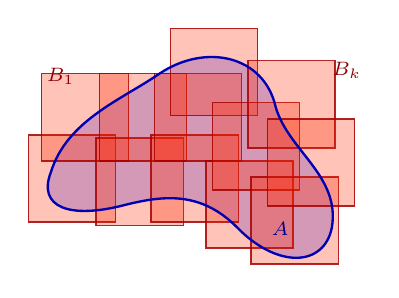
\begin{tikzpicture}[
  scale=0.82,
  every node/.style={font=\scriptsize},
  cover/.style={fill=red!70!orange, fill opacity=0.28, draw=red!65!black, draw opacity=0.85, line width=0.55pt},
  setfill/.style={fill=blue!65, fill opacity=0.34, draw=none},
  setoutline/.style={draw=blue!70!black, line width=0.85pt}
]
  \def\Ashape{%
    (-2.30,-0.42)
      .. controls (-2.05,0.38) and (-1.20,0.70) .. (-0.62,1.10)
      .. controls (0.10,1.58) and (1.00,1.38) .. (1.18,0.58)
      .. controls (1.38,-0.10) and (2.18,-0.48) .. (2.05,-1.28)
      .. controls (1.93,-1.90) and (1.20,-1.92) .. (0.58,-1.28)
      .. controls (0.02,-0.72) and (-0.55,-0.78) .. (-1.18,-0.94)
      .. controls (-2.00,-1.15) and (-2.52,-0.98) .. (-2.30,-0.42)
      -- cycle%
  }

  \path[setfill] \Ashape;

  \foreach \x/\y in {
    -2.65/-1.20,
    -2.45/-0.25,
    -1.60/-1.25,
    -1.55/-0.25,
    -0.75/-1.20,
    -0.70/-0.25,
    -0.45/0.45,
    0.10/-1.60,
    0.20/-0.70,
    0.75/-0.05,
    0.80/-1.85,
    1.05/-0.95
  }{
    \draw[cover] (\x,\y) rectangle ++(1.35,1.35);
  }

  \draw[setoutline] \Ashape;

  \node[blue!55!black] at (1.25,-1.30) {$A$};
  \node[red!55!black] at (-2.15,1.06) {$B_1$};
  \node[red!55!black] at (2.28,1.15) {$B_k$};
\end{tikzpicture}

  \caption{Cover $A\subseteq\bigcup_k B_k$ by squares; minimize $\sum_k\abs{B_k}$.}
  \label{fig:outer-measure-rectangle-cover}
\end{figure}

\begin{perspective} \label{per:outer-measure-geometric-box-covers} \hlt{Outer Measure as Outside Approximation}\\
Outer measure covers $A$ from outside; $d_\mu(A,B)=\mu^\ast(A\triangle B)$ measures closeness.\\
\hlt{Key Insight}: Countable subadditivity collects near-optimal covers.
\end{perspective}

\begin{method} \label{meth:lebesgue-measure-construction} \hlt{Lebesgue Measure Construction}
\begin{enumerate}[label=(\roman*)]
\setlength{\itemsep}{0pt}
\item \hlt{Cover from outside}\\
For $A\subseteq\R^n$, define $m_n^\ast(A)\defeq\inf\left\{\sum_{j\in J}\operatorname{vol}_n(B_j):(B_j)_{j\in J}\text{ covers }A,\ J\text{ at most countable}\right\}$.\\
This is defined for every set, but it is only countably subadditive in general.
\item \hlt{Keep the clean splitters}\\
Call $A$ measurable when every test set $X\subseteq\R^n$ splits additively: $m_n^\ast(X)=m_n^\ast(X\cap A)+m_n^\ast(X\cap A^c)$.\\
These measurable sets form a $\sigma$-algebra.
\item \hlt{Restrict the outer measure}\\
Define Lebesgue measure on measurable sets by $m(A)\defeq m_n^\ast(A)$.\\
On this restricted class, $m$ is countably additive.
\end{enumerate}
\hlt{Key Insight}: Outer measure sizes all sets; clean splitting restores additivity.
\end{method}

\begin{theorem} \label{thm:measure-measurability-main-source-todo}\label{thm:rudin-measure-extension} \hlt{Extension to a Measure}\\
Let $\mu$ be additive, regular, nonnegative, and finite on $\mathcal{E}$. Form $\mu^\ast$ from open elementary covers, set $d_\mu(A,B)=\mu^\ast(A\triangle B)$, and let $\mathcal{M}(\mu)$ be the countable unions of $d_\mu$-limits of elementary sets. Then:
\begin{enumerate}[label=(\roman*)]
\setlength{\itemsep}{0pt}
\item $\mu^\ast(A)=\mu(A)$ for $A\in\mathcal{E}$;
\item $\mu^\ast$ is countably subadditive;
\item $\mathcal{M}(\mu)$ is a $\sigma$-ring;
\item $\mu^\ast$ is countably additive on $\mathcal{M}(\mu)$.
\end{enumerate}
\begin{proof}
\begin{enumerate}[label=(\roman*)]
\setlength{\itemsep}{0pt}
\item Regularity gives $\mu^\ast(A)\leq\mu(A)$; compact closed approximants inside $A$ give the reverse inequality.
\item Cover each $E_n$ within $2^{-n}\varepsilon$ of $\mu^\ast(E_n)$; the combined cover proves subadditivity.
\item If $A_k\to A$, $B_k\to B$ in $d_\mu$, $A_k,B_k\in\mathcal{E}$, then $d_\mu(A_k\diamond B_k,A\diamond B)\leq d_\mu(A_k,A)+d_\mu(B_k,B)\to0$, $\diamond\in\{\cup,\cap,\setminus\}$.\\
Thus $\mathcal{M}_F(\mu)$ is a ring. If $A=\bigcup_kA_k$ with $A_k\in\mathcal{M}_F(\mu)$, then $A\setminus B=\bigcup_k(A_k\setminus B)$, so $\mathcal{M}(\mu)$ is a $\sigma$-ring.
\item For $A=\bigsqcup\limits_n A_n$, $A_n\in\mathcal{M}_F(\mu)$, subadditivity gives $\leq$,\\
while finite additivity gives $\mu^\ast(A)\geq\mu^\ast\left(\bigsqcup\limits_{n=1}^{N}A_n\right)=\sum\limits_{n=1}^{N}\mu^\ast(A_n)$.\\
Let $N\to\infty$, then decompose general disjoint families in $\mathcal{M}(\mu)$ into finite-measurable pieces.
\end{enumerate}
\hlt{Structural Commentary}: Elementary sets are completed under the distance measured by symmetric difference.\\
\hlt{Key Insight}: Approximate by elementary sets, prove identities there, then pass through $d_\mu(A,B)$.
\end{proof}
\end{theorem}

\begin{definition} \label{def:extended-and-lebesgue-measure} \hlt{Extended and Lebesgue Measure}\\
The \hlt{extended measure} is $\mu^\ast|_{\mathcal{M}(\mu)}$, denoted again by $\mu$.\\
For the elementary volume $m$, it is \hlt{Lebesgue measure} on $\R^p$.
\end{definition}

\begin{definition} \label{def:abstract-outer-measure-clean-division} \hlt{Abstract Outer Measure and Clean Division}\\
An \hlt{abstract outer measure} on $M$ is a monotone, countably subadditive function $\omega:2^M\to[0,+\infty]$ with $\omega(\emptyset)=0$.\\
A set $E\subseteq M$ is \hlt{$\omega$-measurable} if it cleanly splits every $X\subseteq M$: $\omega(X)=\omega(X\cap E)+\omega(X\cap E^c)$.\\
For Lebesgue outer measure, this is Caratheodory measurability.
\end{definition}

\begin{lemma} \label{lem:caratheodory-finite-measure-test} \hlt{Finite-Measure Test for Caratheodory Measurability}\\
Let $\omega:2^M\to[0,+\infty]$ be an outer measure. Then $E\subseteq M$ is $\omega$-measurable iff, for all $X\subseteq M$,\\
$\omega(X)<+\infty\Longrightarrow \omega(X)\geq\omega(X\cap E)+\omega(X\cap E^c)$.
\begin{proof}
\begin{enumerate}[label=\roman*.]
\setlength{\itemsep}{0pt}
\item[$(\Rightarrow)$] If $E$ is $\omega$-measurable, then $\omega(X)=\omega(X\cap E)+\omega(X\cap E^c)$ $\forall X\subseteq M$, hence finite-test inequality holds.
\item[$(\Leftarrow)$] For all $X\subseteq M$, $X=(X\cap E)\sqcup(X\cap E^c)$ gives $\omega(X)\leq\omega(X\cap E)+\omega(X\cap E^c)$. If $\omega(X)<+\infty$, the hypothesis gives $\geq$; if $\omega(X)=+\infty$, $\geq$ is automatic in $[0,+\infty]$. Thus equality holds for every $X$.
\end{enumerate}
\hlt{Structural Commentary}: To verify a clean split, only finite outer-measure test sets need real work.\\
\hlt{Key Insight}: Subadditivity supplies one inequality for free.
\end{proof}
\end{lemma}

\begin{figure}[H]
  \centering
  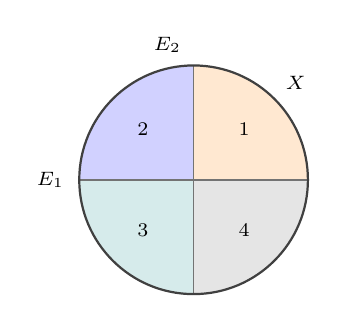
\begin{tikzpicture}[
  scale=0.88,
  every node/.style={font=\scriptsize},
  cut/.style={black!55, line width=0.65pt},
  boundary/.style={black!75, line width=0.8pt}
]
  \begin{scope}
    \clip (0,0) circle (1.65);
    \fill[orange!18] (0,0) rectangle (1.65,1.65);
    \fill[blue!18] (-1.65,0) rectangle (0,1.65);
    \fill[teal!16] (-1.65,-1.65) rectangle (0,0);
    \fill[black!10] (0,-1.65) rectangle (1.65,0);
    \draw[cut] (-1.65,0) -- (1.65,0);
    \draw[cut] (0,-1.65) -- (0,1.65);
  \end{scope}

  \draw[boundary] (0,0) circle (1.65);

  \node at (0.73,0.73) {$1$};
  \node at (-0.73,0.73) {$2$};
  \node at (-0.73,-0.73) {$3$};
  \node at (0.73,-0.73) {$4$};

  \node[above left=1pt] at (0,1.65) {$E_2$};
  \node[left=2pt] at (-1.65,0) {$E_1$};
  \node[above right=1pt] at (1.15,1.12) {$X$};
\end{tikzpicture}

  \caption{Two cuts split $X$ into four regions; $E_1\setminus E_2$ is region $2$.}
  \label{fig:measurable-difference-four-regions}
\end{figure}

\begin{definition} \label{def:outer-measure-zero-sets} \hlt{Zero Sets}\\
For outer measure $\omega:2^M\to[0,+\infty]$, \hlt{$\omega$-zero set} is $Z\subseteq M$ with $\omega(Z)=0$; $\mathcal{Z}_\omega\defeq\{Z\subseteq M:\omega(Z)=0\}$.
\end{definition}

\begin{theorem} \label{thm:caratheodory-measurable-sets-sigma-algebra} \hlt{Caratheodory Measurable Sets}\\
Let $\omega:2^M\to[0,+\infty]$ be an outer measure, and let $\mathcal{M}_\omega$ be the class of $\omega$-measurable subsets of $M$.\\
Then $\mathcal{M}_\omega$ is a $\sigma$-algebra, $\omega|_{\mathcal{M}_\omega}$ is countably additive, $\mathcal{Z}_\omega\subseteq\mathcal{M}_\omega$, and $E\in\mathcal{M}_\omega$, $Z\in\mathcal{Z}_\omega$\\
imply $E\cup Z,E\setminus Z,E\triangle Z\in\mathcal{M}_\omega$ and $\omega(E\cup Z)=\omega(E\setminus Z)=\omega(E\triangle Z)=\omega(E)$.
\begin{proof}
If $Z\in\mathcal{Z}_\omega$, then $\omega(X)\leq\omega(X\cap Z)+\omega(X\cap Z^c)\leq0+\omega(X)$, so $Z\in\mathcal{M}_\omega$. Complements are immediate.\\
If $E,F\in\mathcal{M}_\omega$, iterating the two clean cuts gives $\omega(X)=\sum_{\epsilon,\eta\in\{0,1\}}\omega(X\cap E^\epsilon\cap F^\eta)$, where $E^1=E$, $E^0=E^c$; hence all finite Boolean combinations of $E,F$ are measurable.\\
For disjoint $E_i\in\mathcal{M}_\omega$, set $E=\bigsqcup_iE_i$ and $F_N=(\bigcup_{i=1}^{N}E_i)^c$.\\
Finite splitting gives $\omega(X)=\sum_{i=1}^{N}\omega(X\cap E_i)+\omega(X\cap F_N)\geq\sum_{i=1}^{N}\omega(X\cap E_i)+\omega(X\cap E^c)$.\\
Letting $N\to\infty$ and using subadditivity for the reverse inequality yields $\omega(X)=\sum_{i=1}^{\infty}\omega(X\cap E_i)+\omega(X\cap E^c)$; hence $E\in\mathcal{M}_\omega$, and $X=E$ gives countable additivity.\\
General countable unions follow from $F_1=E_1$, $F_n=E_n\setminus\bigcup_{i<n}E_i$.\\
Finally, if $E\in\mathcal{M}_\omega$ and $Z\in\mathcal{Z}_\omega$, then $E=(E\setminus Z)\sqcup(E\cap Z)$ and $E\cup Z=E\sqcup(Z\setminus E)$ give $\omega(E\setminus Z)=\omega(E)$ and $\omega(E\cup Z)=\omega(E)$; also $E\triangle Z=(E\setminus Z)\sqcup(Z\setminus E)$ has measure $\omega(E)$.\\
\hlt{Structural Commentary}: Measurable sets preserve countable additivity.\\
\hlt{Key Insight}: Measurable cuts turn subadditivity into equality.
\end{proof}
\end{theorem}

\begin{definition} \label{def:lebesgue-sigma-algebra-caratheodory} \hlt{Lebesgue $\sigma$-Algebra via Caratheodory}
\begin{enumerate}[label=(\roman*)]
\setlength{\itemsep}{0pt}
\item $\mathcal{L}^n\defeq\{E\subseteq\R^n:E$ is $m_n^\ast$-measurable$\}$ is the \hlt{Lebesgue $\sigma$-algebra}.
\item $m\defeq m_n^\ast|_{\mathcal{L}^n}$ is \hlt{Lebesgue measure}; for $E\in\mathcal{L}^n$, write $m(E)=m_n^\ast(E)$.
\end{enumerate}
\end{definition}

\begin{proposition} \label{prop:cells-lebesgue-measurable-volume} \hlt{Cells Are Lebesgue Measurable}\\
For every coordinate cell $I\subseteq\R^n$, $I\in\mathcal{L}^n$ and $m(I)=\operatorname{vol}_n(I)$.
\begin{proof}
Since $I\in\mathcal{E}$, Theorem \ref{thm:rudin-measure-extension} gives $I\in\mathcal{L}^n$ and $m(I)=m_n^\ast(I)=\operatorname{vol}_n(I)$.\\
For the open-cell split, fix $A\subseteq\R^n$ with $m_n^\ast(A)<+\infty$.\\
Set $I_k\defeq\{x\in I:\operatorname{dist}(x,I^c)>k^{-1}\}$, $\eta_k\defeq m_n^\ast(I\setminus I_k)\to0$. Since $\operatorname{dist}(A\cap I_k,A\setminus I)>0$, Theorem \ref{thm:outer-measure-positive-distance-additivity} gives $m_n^\ast(A)\geq m_n^\ast(A\cap I_k)+m_n^\ast(A\setminus I)\geq m_n^\ast(A\cap I)+m_n^\ast(A\setminus I)-\eta_k$; let $k\to\infty$ and apply Lemma \ref{lem:caratheodory-finite-measure-test}.\\
\hlt{Structural Commentary}: Cells are the bridge between coordinate volume and Lebesgue measure.\\
\hlt{Key Insight}: Shrink, split, let the collar vanish.
\end{proof}
\end{proposition}
